\documentclass{../template/myrpt}
\usepackage{tabularray}

\usepackage{fancyhdr}
\usepackage{xcolor}

\UseTblrLibrary{booktabs}

\ExamName{弗朗克赫兹实验}

\begin{document}
\maketitle

\section{实验目的}
\begin{enumerate}
  \item 本实验通过对氩原子第一激发电位的测量，了解弗兰克和赫兹研究原子内部能量量子化的基本思想和方法；
  \item 了解电子与原子碰撞和能量交换过程的微观图像，以及影响这个过程的主要物理因素。
\end{enumerate}

\section{实验仪器}

\begin{figure}[htbp]
  \centering
  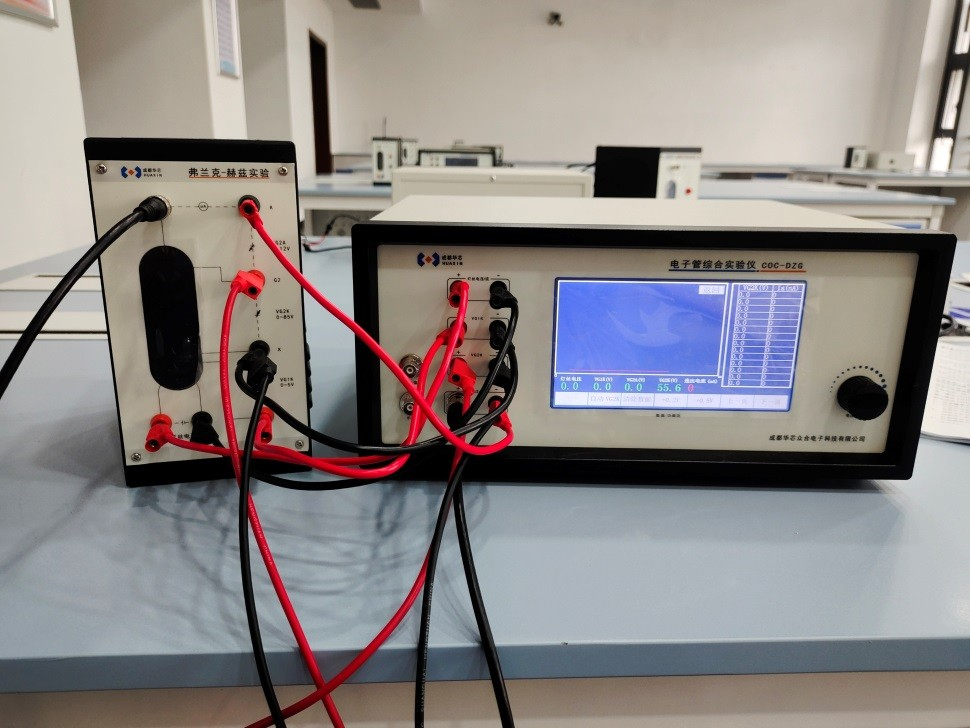
\includegraphics[width=0.5\linewidth]{assets/弗兰克赫兹实验仪器.jpg}
  \caption{电子管综合实验仪、弗兰克赫兹实验仪}
\end{figure}

\section{实验原理}

\subsection{玻尔原子理论}
根据玻尔的原子理论，原子只能较长久地停留在一些稳定的状态下，简称“定态”。原子在定态时既不发射能量也不吸收能量，各定态的能量是分立的，即处于不同的能级上。原子只能吸收或辐射出相当于各能级之间差值的能量：
$$ \Delta E = E_2 - E_1 = h\nu $$
其中 $h$ 为普朗克常数，$\nu$ 为辐射频率。要使原子状态改变，必须有外部能量作用。本实验通过加速电子，使具有一定能量的电子与原子碰撞进行能量交换而实现原子能态的改变。

\subsection{弗兰克-赫兹实验原理与装置}
实验装置主要由充气（如氩气）电子管组成，包含阴极 $K$、第一栅极 $G_1$、第二栅极 $G_2$ 和阳极 $A$。

\begin{figure}[htbp]
  \centering % 保持整体居中
  \begin{minipage}[c]{0.27\linewidth}
    \centering
    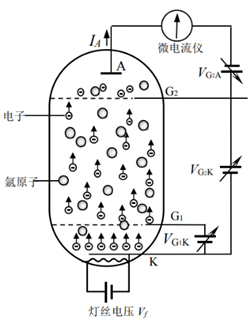
\includegraphics[width=\linewidth]{assets/实验装置图.png}
    \caption{实验原理示意图}\label{fig:show1}
  \end{minipage}
  \hspace{1em} % 添加一点水平间距，防止图片紧贴
  \begin{minipage}[c]{0.45\linewidth}
    \centering
    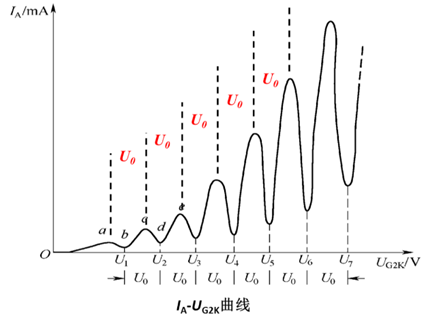
\includegraphics[width=\linewidth]{assets/I_A-U_G2K曲线.png}
    \caption{$I_A\sim V_{G_2K}$ 曲线}
    \label{fig:show2}
  \end{minipage}
\end{figure}

如图 \ref{fig:show1} 所，其中 $V_{G_1K}$ 的作用是消除空间电荷对阴极电子发射的影响，提高发射效率；
   $V_{G_2K}$ 为加速电压，为电子提供能量；
   $V_{G_2A}$ 为拒斥电压，在 $G_2$ 与阳极 $A$ 之间形成反向电场。

当电子能量小于氩原子的第一激发能时，电子基本不损失动能，碰撞为弹性碰撞；当电子能量达到第一激发能 $eU_0=h\nu=\Delta E$ 的临界能量时，那么，当电子与原子发生非弹性碰撞时，原子会吸收电子能量从基态跃迁到第一激发态。相应的电位差 $U_0$ 也称为氩原子的第一激发电位。当电子的能量等于或大于第一激发能的时候，原子就开始发光。

如图 \ref{fig:show2} 在达到临界能量之前，电子经过 $K$ 至 $G_2$ 加速，随加速电压 $V_{G_2K}$ 增加，越来越多的电子具有足够的能量克服拒斥电场作用到达阳极，使电流 $I_A$ 增大。当电子能量达到临界能量足以使原子激发后，剩余动能不足以克服拒斥电场 $V_{G_2A}$，导致 $I_A$ 下降，形成峰值。随着电子能量进一步增大，电子在进入拒斥电场前可能发生了多次碰撞，从而形成多个阳极电流峰值，相邻两个峰值对应的电压差为原子的第一激发电位 $U_0$
$$ \Delta V_{G_2K} = U_0 $$

\section{实验内容和步骤}

\subsection{测量氩原子的第一激发电位}
通过绘制 $I_A \sim V_{G_2K}$ 曲线，观察原子能量量子化情况，并求出第一激发电位。

\begin{minipage}[t]{0.57\linewidth} % 左侧文字部分，占 65% 宽度
\textbf{1.} 按照图1.2b连接好实验电路，接通电源。\\
\textbf{2.} 主机启动后，在弗兰克——赫兹实验主菜单中点击“左边第一栏”进行参数设置，设置以下参数：灯丝电压 $V_f=2.2V$、第一栅极电压 $V_{G_1K}=1.5V$、拒斥电压 $V_{G_2A}=9.0V$。\\
\textbf{3.} 预热3分钟，点击弗兰克——赫兹实验主菜单的“自动模式”，开始进行“自动模式”实验，仪器控制 $V_{G_2K}$ 从 0V 到 85V 以 0.2V 的步距绘制$I_A \sim V_{G_2K}$ 曲线，并将实验数据保存。\\
\end{minipage}
\hspace{0.02\linewidth}
\hfill
\begin{minipage}[t]{0.35\linewidth} % 右侧图片部分，占 30% 宽度
  \vspace{-10pt} % 确保图片与第一行文字对齐
  \centering
  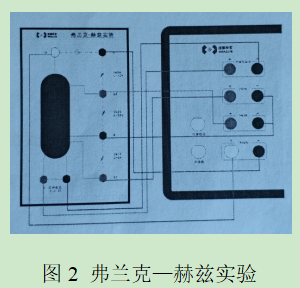
\includegraphics[width=\linewidth]{assets/弗兰克实验连接图.png}
\end{minipage}

\begin{minipage}[t]{0.95\linewidth}
\textbf{4.} 注观察屏上曲线形态，若曲线削峰，适当降低灯丝电压 $V_f$ ；若削谷，适当降低拒斥电压 $ V_{G_2A}$ 。重新开始，直到绘制出包括6个完好的峰和谷的$I_A \sim V_{G_2K}$ 曲线。\\
\textbf{5.} 在弗兰克——赫兹实验主菜单，点击右边“下一页”进行数据查询，屏幕上列出最近一次自动模式测量的数据，在数据列表中找到电流 $I_A$ 的每一个峰和谷值，记录极值电流对应的速电压 $V_{G_2K}$ 填入表 \ref{table1}。
  
\end{minipage}

\newcolumntype{Y}{>{\centering\arraybackslash}X}
% 注：如果在导言区没有定义 C 列，请添加以下定义：
\newcolumntype{C}{>{\centering\arraybackslash}X}

\begin{LabRecordTable}
% \begin{table}[htbp]
\centering
\caption{自动模式 $I_A \sim V_{G_2K}$ 曲线峰、谷电压记录}
\label{table1}
\setlength{\tabcolsep}{3pt} % 适当减小列间距以压缩整体宽度
\begin{tabularx}{\textwidth}{c *{6}{C} *{3}{c} C} % 使用自定义的C列或c列
\toprule
% 使用 \mbox 确保序号不换行
{序号 $i$} & 1 & 2 & 3 & 4 & 5 & 6 
& \multicolumn{3}{c}{$V_{i+3}-V_i$/V} 
& \mbox{平均值} \\
\midrule
峰 $V_{G_2K}$/V & 19.8 & 30.8 & 42.2 & 54.2 & 65.8 & 78.6 & 34.4 & 35.0 & 36.4 & 35.3 \\
谷 $V_{G_2K}$/V & 24.8 & 36.6 & 48.8 & 60.0 & 72.2 & --- & 35.2 & 35.6 & --- & 35.4 \\
\bottomrule
\end{tabularx}
% \end{table}
\end{LabRecordTable}

由表 \ref{table1} 中峰、谷电压值，采用逐差法计算氩原子的第一激发电位：
\[
  U_0 = \frac{V_{i+3}-V_i}{3}
\]
由峰值计算得到
\[
  U_{0,\text{峰}} = \frac{34.4 + 35.0 + 36.4}{3 \times 3} = 11.76\ \text{V}
\]
由谷值计算得到
\[
  U_{0,\text{谷}} = \frac{35.2 + 35.6}{2 \times 3} = 11.80\ \text{V}
\]
取氩原子第一激发电位公认值 $U_{0\text{ref}} = 11.6\ \text{V}$，则峰值法与谷值法的相对误差分别为
\[
  \eta_{\text{峰}} = \frac{|11.76 - 11.6|}{11.6} \times 100\% = 1.35\%
\]
\[
  \eta_{\text{谷}} = \frac{|11.80 - 11.6|}{11.6} \times 100\% = 1.72\%
\]
综合峰、谷两组结果，可认为本实验测得氩原子的第一激发电位约为 $11.77\ \text{V}$。

\section{实验的分析和总结}

自动模式下测得的 $I_A \sim V_{G_2K}$ 曲线具有较明显的周期性峰谷结构。随着加速电压 $V_{G_2K}$ 增大，电子获得的动能逐渐增大；当电子动能达到氩原子的第一激发能时，电子与氩原子发生非弹性碰撞，将部分能量传递给原子，使电子自身剩余动能减小，难以克服拒斥电场到达阳极，因而阳极电流下降并形成谷值。继续增大加速电压后，电子重新获得足够动能，阳极电流再次上升，于是曲线呈现出周期性的峰谷变化。

由表 \ref{table1} 可见，无论取峰值还是谷值，$V_{i+3}-V_i$ 都接近常数，说明相邻三个峰或谷之间对应的总电压增量近似固定。这表明电子在管内重复经历“加速获得能量、与氩原子非弹性碰撞失去约一个激发能、再继续加速”的过程，反映出氩原子只能吸收特定大小的能量，即原子的能级是分立的，弗兰克-赫兹实验因此为原子能级量子化提供了直接证据。

采用逐差法处理数据后，峰值法得到的第一激发电位为 $11.76\ \text{V}$，谷值法得到的第一激发电位为 $11.80\ \text{V}$，两者与公认值 $11.6\ \text{V}$ 都较为接近，相对误差分别为 $1.35\%$ 和 $1.72\%$。这说明本次实验测量结果可信，实验装置工作正常，所测曲线能够较好反映氩原子第一激发电位的物理意义。

实验误差主要可能来自以下几个方面：一是从自动模式曲线中读取峰、谷对应电压时存在有限分辨率和人工判读误差；二是电子在电子管中的初速度分布、空间电荷效应以及气体压强变化会使峰谷位置发生轻微偏移；三是拒斥电压、灯丝电压和仪器稳定性也会影响曲线形状，从而影响极值点判断。总体来看，这些因素未改变周期结构的基本规律，因此不影响对氩原子第一激发电位的测定结论。

\insertSignedDataPage

\end{document}
